\scalebox{0.95}{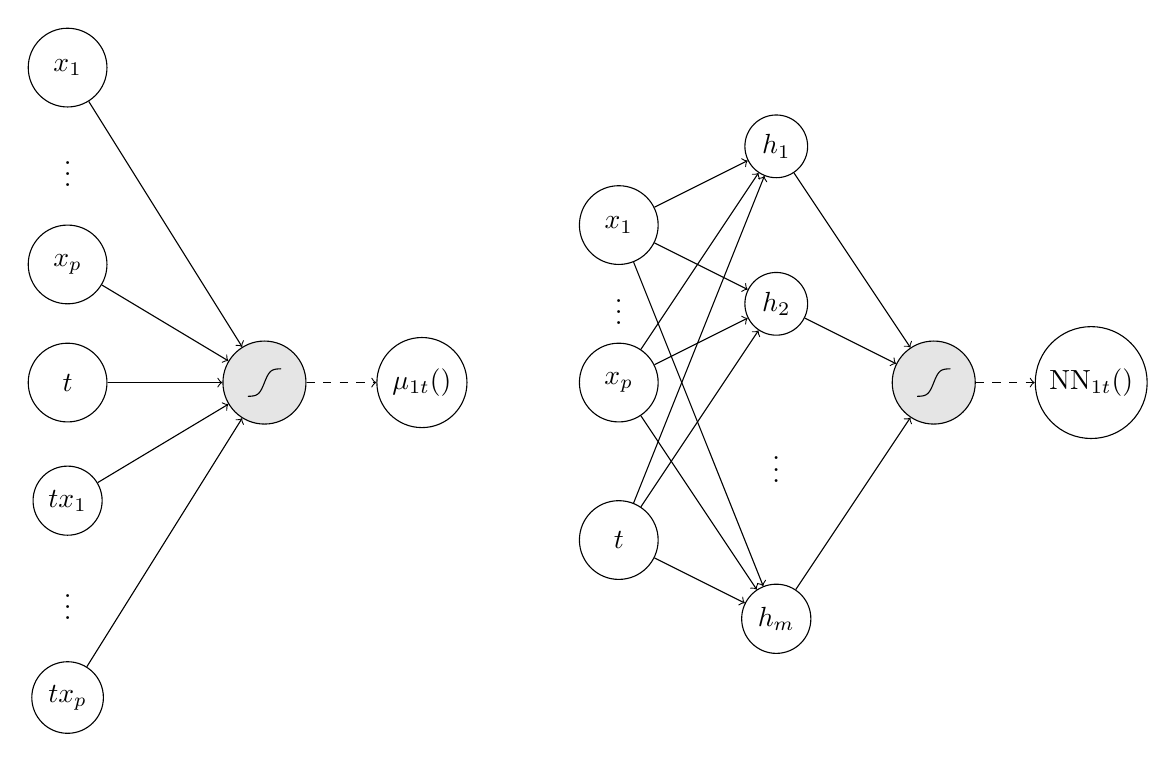
\begin{tikzpicture}
    
    
    \tikzset{dist/.style={path picture= {
    \begin{scope}[x=1pt,y=10pt]
      \draw plot[domain=-6:6] (\x,{1/(1 + exp(-\x))-0.5});
    \end{scope}
    }}}
    \tikzstyle{sigmoid}=[draw,fill=gray!20,circle,minimum size=30pt,inner sep=0pt,dist]
    
    % Interaction Model
    % INPUT LAYER
    % T=1
    %\draw[red,thick,dashed] (0,3) circle (5mm);
    \node(x11) at (0,3) [circle, draw, minimum size=1cm] {$x_1$};
    \node at (0,1.75) {$\vdots$};
    %\draw[red,thick,dashed] (0,0.5) circle (5mm);
    \node(x1p) at (0,0.5) [circle, draw, minimum size=1cm] {$x_p$};
    %\draw[blue,thick,dashed] (0,-1) circle (5mm);
    \node(t1) at (0,-1) [circle, draw, minimum size=1cm] {$t$};
    %\draw[blue,thick,dashed] (0,-2.5) circle (5mm);
    \node(t1x11) at (0,-2.5) [circle, draw] {$t x_1$};
    \node at (0,-3.75) {$\vdots$};
    %\draw[blue,thick,dashed] (0,-5) circle (5mm);
    \node(t1x1p) at (0,-5) [circle, draw] {$t x_p$};
   
    % CONDITIONAL MEAN 
    \node (p1)[sigmoid] at (2.5, -1) {};
    
    % WEIGHTS
    \draw[->] (x11) -- (p1) node [midway,above] {};%{$\beta_1$};
    \draw[->] (x1p) -- (p1) node [midway,above] {};%{$\beta_p$};
    \draw[->] (t1) -- (p1) node [midway,above] {};%{$\gamma$};
    \draw[->] (t1x11) -- (p1) node [midway,above] {};%{$\delta_1$};
    \draw[->] (t1x1p) -- (p1) node [midway,above] {};%{$\delta_p$};
    
    % OUTPUT
    %\draw[black] (4.5,-1) circle (7mm);
    \node(mu1t) at (4.5,-1) [circle, draw] {$\mu_{1t}(\x)$};
    \draw[->, dashed] (p1) -- (mu1t);
    
    % Neural Net
    % INPUT LAYER
    % T=1
    %\draw[red,thick,dashed] (7,1) circle (5mm);
    \node(x11) at (7,1) [circle, draw, minimum size=1cm] {$x_1$};
    \node at (7,0) {$\vdots$};
    %\draw[red,thick,dashed] (7,-1) circle (5mm);
    \node(x1p) at (7,-1) [circle, draw, minimum size=1cm] {$x_p$};
    %\draw[blue,thick,dashed] (7,-3) circle (5mm);
    \node(t1) at (7,-3) [circle, draw, minimum size=1cm] {$t$};

    % HIDDEN LAYER
    % T=1
    %\draw[black,thick,dashed] (9,2) circle (5mm);
    \node(h11) at (9,2) [circle, draw] {$h_1$};
    %\draw[black,thick,dashed] (9,0) circle (5mm);
    \node(h12) at (9,0) [circle, draw] {$h_2$};
    \node at (9,-2) {$\vdots$};
    %\draw[black,thick,dashed] (9,-4) circle (5mm);
    \node(h1m) at (9,-4) [circle, draw] {$h_m$};
    
    % CONDITIONAL MEAN
    \node (p1)[sigmoid] at (11, -1) {};

    % WEIGHTS
    %1st layer T=1
    \draw[->] (x11) -- (h11) node [midway,above] {};
    \draw[->] (x1p) -- (h11) node [midway,above] {};
    \draw[->] (t1) -- (h11) node [midway,above] {};
    
    \draw[->] (x11) -- (h12) node [midway,above] {};
    \draw[->] (x1p) -- (h12) node [midway,above] {};
    \draw[->] (t1) -- (h12) node [midway,above] {};
    
    \draw[->] (x11) -- (h1m) node [midway,above] {};
    \draw[->] (x1p) -- (h1m) node [midway,above] {};
    \draw[->] (t1) -- (h1m) node [midway,above] {};


    %2nd layer
    \draw[->] (h11) -- (p1) node [midway,above] {};
    \draw[->] (h12) -- (p1) node [midway,below] {};
    \draw[->] (h1m) -- (p1) node [midway,below] {};

    
    % OUTPUT
    %\draw[black] (13,-1) circle (7mm);
    \node(mu1t) at (13,-1) [circle, draw] {$\mathrm{NN}_{1t}(\x)$};
    \draw[->, dashed] (p1) -- (mu1t);
    
    
    
\end{tikzpicture}}
